\documentclass{amsart}
\synctex=1

%=================================================================
% 
\newcount\DraftStatus  % 0 suppresses notes to selves in text
\DraftStatus=1   % TODO: set to 0 for final version
%=================================================================

%=================================================================
\usepackage{comment}
%=================================================================
%
\includecomment{JournalOnly}  
\includecomment{ConferenceOnly}  
\includecomment{TulipStyle}
%
%=================================================================
%=================================================================
% gitlatexdiff
%
%  https://gitlab.com/git-latexdiff/git-latexdiff
%=================================================================
%  git latexdiff HEAD  HEAD~5 --main templatex.tex
%  git latexdiff HEAD~1  --main templatex.tex
%  View pdf to see difference
%
%=================================================================
%
% Todo Notes for marginal comments
% 
%\newcount\DraftStatus  % 0 suppresses notes to selves in text
%\DraftStatus=1   % TODO: set to 0 for final version
\ifnum\DraftStatus=1
	\usepackage[draft,colorinlistoftodos,color=orange!30]{todonotes}
\else
	\usepackage[disable,colorinlistoftodos,color=blue!30]{todonotes}
\fi 
%\usepackage[disable]{todonotes} % notes not showed
%\usepackage[draft]{todonotes}   % notes showed
%
\makeatletter
 \providecommand\@dotsep{5}
 \def\listtodoname{List of Todos}
 \def\listoftodos{\@starttoc{tdo}\listtodoname}
 \makeatother
%
%=================================================================
%
\usepackage{color}
\newcommand{\draftnote}[3]{ 
	\todo[author=#2,color=#1!30,size=\footnotesize]{\textsf{#3}}	}
% TODO: add yourself here:
%
\newcommand{\gangli}[1]{\draftnote{blue}{GLi:}{#1}}
\newcommand{\qwu}[1]{\draftnote{red}{QWu:}{#1}}
\newcommand{\gliMarker}
	{\todo[author=GLi,size=\tiny,inline,color=blue!40]
	{Gang Li has worked up to here.}}
\newcommand{\qwuMarker}
	{\todo[author=QWu,size=\tiny,inline,color=red!40]
	{Qiong Wu has worked up to here.}}
%=================================================================

%=================================================================
%
% general packages
%  https://en.wikibooks.org/wiki/Category:Book:LaTeX
%  https://en.wikibooks.org/wiki/LaTeX/Package_Reference
%
%=================================================================
\usepackage{graphicx}
\usepackage{algorithm}
\usepackage{algorithmic}
\usepackage{breqn}
\usepackage{subcaption}
\usepackage{multirow}
\usepackage{psfrag}
\usepackage{url}
\usepackage{hyperref}
%\usepackage[colorlinks]{hyperref}
%\usepackage{cite}
\usepackage{cleveref}
\usepackage{booktabs}
\usepackage{rotating}
\usepackage{colortbl}
\usepackage{paralist}
%\usepackage{geometry}
\usepackage{epstopdf}
\usepackage{nag}
\usepackage{microtype}
\usepackage{siunitx}
\usepackage{nicefrac}
% for random text
\usepackage{lipsum}
\usepackage[english]{babel}
\usepackage[pangram]{blindtext}
% for tikz figures
\usepackage{tikz}
\usetikzlibrary{fit,positioning,arrows.meta,shapes,arrows}
%\tikzset{neuron/.style={circle,thick,fill=black!25,minimum size=17pt,inner sep=0pt},
%	input neuron/.style={neuron, draw,thick, fill=gray!30},
%	hidden neuron/.style={neuron,fill=white,draw},
%	hoz/.style={rotate=-90}}
%
%=================================================================



\begin{TulipStyle}
\usepackage[numbers]{natbib}
%=================================================================
%
% Version control information
%
%=================================================================
\usepackage{gitinfo2}
%=================================================================
\usepackage{fancyhdr}
\pagestyle{fancy}
\fancyhead{} % clear all header fields
\fancyhead[RO,LE]{\textsl{\rightmark}}
\fancyhead[LO,RE]{\ensuremath{\Rightarrow}
		\textbf{\textbf{[CONFIDENTIAL]}}\ensuremath{\Leftarrow}}
\fancyhead[CO,CE]{}
%=================================================================
\fancyfoot{} % clear all footer fields
\fancyfoot[CE,CO]{\textbf{\thepage}} 
\fancyfoot[LO,LE]{
\includegraphics[height=.9\headheight]{logos/tulip-logo.eps}
		flip01-develop(2021-1-16)}
\fancyfoot[RO,RE]{Committed by: \textsl{Baobao Song}}

\setlength{\headheight}{12pt}
\renewcommand{\headrulewidth}{0.4pt}
\renewcommand{\footrulewidth}{0.4pt}
%=================================================================


%=================================================================
% for math notations
% ----------------------------------------------------------------
\usepackage{mathtools}
\usepackage{amsthm}
%
% THEOREMS -------------------------------------------------------
%
\newtheorem{thm}{Theorem}[section]
\newtheorem{cor}[thm]{Corollary}
\newtheorem{lem}[thm]{Lemma}
\newtheorem{prop}[thm]{Proposition}
\theoremstyle{definition}
\newtheorem{defn}[thm]{Definition}
\theoremstyle{remark}
\newtheorem{rem}[thm]{Remark}
\numberwithin{equation}{section}
% MATH -----------------------------------------------------------
\newcommand{\norm}[1]{\left\Vert#1\right\Vert}
\newcommand{\abs}[1]{\left\vert#1\right\vert}
\newcommand{\set}[1]{\left\{#1\right\}}
\newcommand{\Real}{\mathbb R}
\newcommand{\eps}{\varepsilon}
\newcommand{\To}{\longrightarrow}
\newcommand{\BX}{\mathbf{B}(X)}
% ----------------------------------------------------------------
\newcommand{\I}{{\cal I}}
\newcommand{\Id}{{\cal I} }
\newcommand{\Dc}{{\cal D}}
\newcommand{\J}{{\cal J}}
\newcommand{\Dn}{{\cal D}_n}
\newcommand{\Dd}{{\cal D}_n }
\renewcommand{\P}{{\cal P}}
\newcommand{\Nu}{{\cal N} }
\newcommand{\B}{{\cal B}}
\newcommand{\Bf}{{\bf B}}
\newcommand{\Y}{{\bf Y}}
\newcommand{\A}{{\cal A}}
% ----------------------------------------------------------------
\newcommand{\V}{{\cal V}}
\newcommand{\M}{{\cal M}}
\newcommand{\F}{{\cal F}}
\newcommand{\Fd}{{\cal F}}
\newcommand{\BF}{{\cal BF}_n}
\newcommand{\BFd}{{\cal BF}_n}
\newcommand{\TF}{{\cal TF}_n}
\newcommand{\TFd}{{\cal TF}_n}
%\newcommand{\G}{{\cal G}}
\newcommand{\X}{{\cal X}}
\newcommand{\E}{{\cal E}}
\newcommand{\K}{{\cal K}}
\newcommand{\T}{{\cal T}_n}
\renewcommand{\H}{{\cal H}}
% ----------------------------------------------------------------
\newtheorem{Remark}{Remark}
\newtheorem{proposition}{Proposition}
\newtheorem{theorem}{Theorem}
\newtheorem{lemma}{Lemma}
\newtheorem{corollary}{Corollary}
\newtheorem{example}{Example}
\newtheorem{definition}{Definition}
\newtheorem{Algorithms}{Algorithm}
% ----------------------------------------------------------------
\newcommand{\bu}{{\mathbf 1} }
\newcommand{\bo}{{\mathbf 0} }
\newcommand{\N}{\mbox{{\sl l}}\!\mbox{{\sl N}}}
% ----------------------------------------------------------------
\def\uint{[0,1]}
\def\proof{{\scshape Proof}. \ignorespaces}
\def\endproof{{\hfill \vbox{\hrule\hbox{%
   \vrule height1.3ex\hskip1.0ex\vrule}\hrule
  }}\par}
%
%=================================================================

\hypersetup
{
    pdfauthor={\gitAuthorName},
    pdfsubject={TULIP Lab},
    pdftitle={},
    pdfkeywords={TULIP Lab, Data Science},
%	bookmarks=true,  
}

\end{TulipStyle}




%=================================================================
%
\begin{document}
%
%=================================================================
% Preamble which will need to be changed for submission
%
\title[A Short Running Title]{Title of This Paper}%

\author{Author 1}
\address[A.~1]{School of Computer Science,\\ 
Xi'an Shiyou University, Shaanxi 710065, China}%
\email[A.~1]{xxx@tulip.academy}

\author{Gang Li}
\address[A.~2]{School of Information Technology \\
Deakin University, Geelong, Australia}%
\email[A.~2]{gang.li@deakin.edu.au}

\author{Author 3}
\address[A.~3]{School of Information Technology \\
Deakin University, 221 Burwood Highway \\
Vic 3125, Australia}%
\email[A.~3]{xxx@deakin.edu.au}

%\thanks{Thanks to \ldots}%
\subjclass{Artificial Intelligence}%
\keywords{Machine Learning, Data Mining, ...}%
\date{\gitAuthorDate}%

\begin{abstract}
The abstract will be put here, ....
\end{abstract}

\maketitle
\tableofcontents

\newpage
%=================================================================

%=================================================================
\section{Introduction}\label{sec-intro}
\subsection{Problem Describtion}
\smallskip
The Home Depot wants to solve the problem that search result matches the search query. They gives some data about the relevance scores which users rated and we need to predict the scores between search words and product id. The raw dataset contains train set with 74067 samples and test set with 166693 samples which need to write relevance score. Some other information such as product title also provide.
\subsection{Dataset Interpretation}
\smallskip
Here's the data in the dataset.\\
\bigskip
\centerline{\normalsize{Table 1:Data}}
	\begin{tabular}{cp{8cm}<{\centering}p{14cm}<{\centering}}
		\hline
		Name&Attribute\\
		\hline
		train.csv& id, product_id, product_title,search_term, relevance\\
		test.csv& id, product_id, product_title,search_term\\
		product_descriptions.csv& product_uid,product_description\\
		attributes.csv& product_uid,name,value\\
		relevance_instructions.doc& rate the relevance of a search result \\
		sample_submission.csv& id,relevance\\
		\hline
	\end{tabular}
\subsection{Evaluation Criteria}
Home Depot have the score ranking of the test set which users have done before. Therefore, by predicting the relevanca score, MSE methods are used to evaluate the model performance.
Before experiment,  the evaluation methods to assess the model performance is very important, usually it has the MSE methods to evaluate.
\section{Text Preprocessing} \label{sec-preliminaries}	
\subsection{Punctuation and Stopword Removment} Before removing puctuation and stopwords, the test set and train set need to merge and concat the column of product description. Then the punctuations are removed besides ".", "/", -", " \% " because they may have some useful purpose. Next,uppercase is convertes to lowercase and  Arabic numerals arechanged. Finally, stopwords are removed. The results are shown in the figure 1.

\begin{figure}[htb]
	\centering
	\includegraphics[width=13cm, height=8cm]{figures/stop.eps}\\
	\caption{Punctuations and Stopwords are removed in the dataset 
	}\label{straddltimeScale}
\end{figure}
\subsection{Stemming} Using SnowballStemmer to extract stem of text and results are shown in the figure 2.
\begin{figure}[htb]
	\centering
	\includegraphics[width=13cm, height=8cm]{figures/stem.eps}
	\caption{Usage of SnowballStemmer
	}\label{straddltimeScale}
\end{figure}

\section{Text Feature} \label{sec-method}
\subsection{Fundamental Feature}	
Fundamental Features can directly get in the dataset,and it is the visual representation of relevance. Fundamental features are shown below and the code results is in figure 3.
\begin{itemize}
	\item the length of search term
	\item the number of same keywords between search terms and product title 
	\item the number of same keywords between search terms and product description
\end{itemize}
	\begin{figure}[htb]
	\centering
	\includegraphics[width=13cm, height=8cm]{figures/same.eps}
	\caption{Fundamental Feature in Database
	}\label{straddltimeScale}
\end{figure}


\subsection{Levenshtein Distance}
Levenshtein Distance means the times that one string change to another string. Therefore, Levenshtein Distance is used to measure the similarity between search words and other information about product.The features 
	\smallskip
\\of Levenshtein distance are shown below and the code results is in figure 4.
\begin{itemize}
	\item Levenshtein text similarity between search term and product title
	\item Levenshtein text similarity between search term and product
\end{itemize}
	\begin{figure}[htb]
	\centering
	\includegraphics[width=13cm, height=6cm]{figures/leve.eps}
	\caption{Levenshtein Distance features
	}\label{straddltimeScale}
\end{figure}

\subsection{TF-IDF}
First we set a new column named all_text which includes all words in dataset and make a corpus. Then, bag-of-words is used to change words into vectors. Finally, we should calculate the similarity of different sentence. And expand the sentence size to dictionary size and put zero in the position which don't have strings before. In this part, two new feature are created at the result is shown in the figure 5.

\begin{itemize}
	\item Cosine similarity between search terms and product title
	\item Cosine similarity between search terms and product description
\end{itemize}
\begin{figure}[htb]
	\centering
	\includegraphics[width=13cm, height=6cm]{figures/tfidf.eps}
	\caption{TF-IDF features
	}\label{straddltimeScale}
\end{figure}

\subsection{Word2Vec}
Word2Vec assigns a value to each word according to sentences and the context. So, we need to split the sentences from all_test and then split the word. Finally, the value of words we get and then calculate average vector according to sentences, and gain cosine similarity of two sentences.Two new feature are created at the result is shown in the figure 6.
\begin{itemize}
	\item Cosine similarity between search terms and product title
	\item Cosine similarity between search terms and product description
\end{itemize}

\begin{figure}[htb]
	\centering
	\includegraphics[width=13cm, height=6cm]{figures/word2vec.eps}
	\caption{Word2Vec features
	}\label{straddltimeScale}
\end{figure}

\section{Modeling and Forecasting} \label{sec-experiment}
\noindent Using different models to predict the relevance and choose the best one. Bagging Regression, Gradient Boost Regression and Random Forest Regression are compared.In each method, adjusting parameters include max depth and iterations. CV error is used to judge the model performance and its scoring is MSE. At the end,  Gradient Boost Regression performance is best, Random Forest Regression is second and Bagging Regression is last. Parameters adjustment processes of Gradient Boost Regression are shown in figure 7 and 8.  


\begin{figure}[htb]
	\centering
	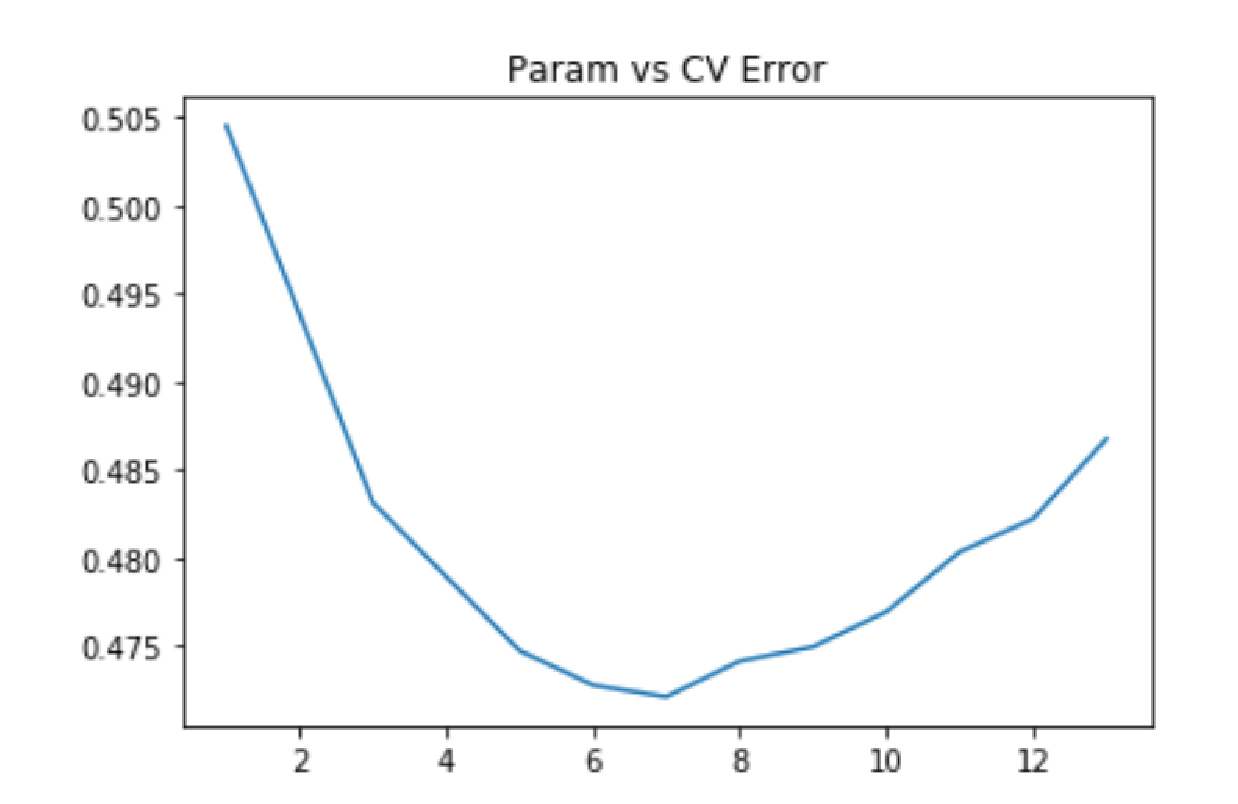
\includegraphics[width=10cm, height=5cm]{figures/adjust3.eps}
	\caption{Adjusting max depth of Gradient Boosting Regressor
	}\label{straddltimeScale}
\end{figure}
\begin{figure}[htb]
	\centering
	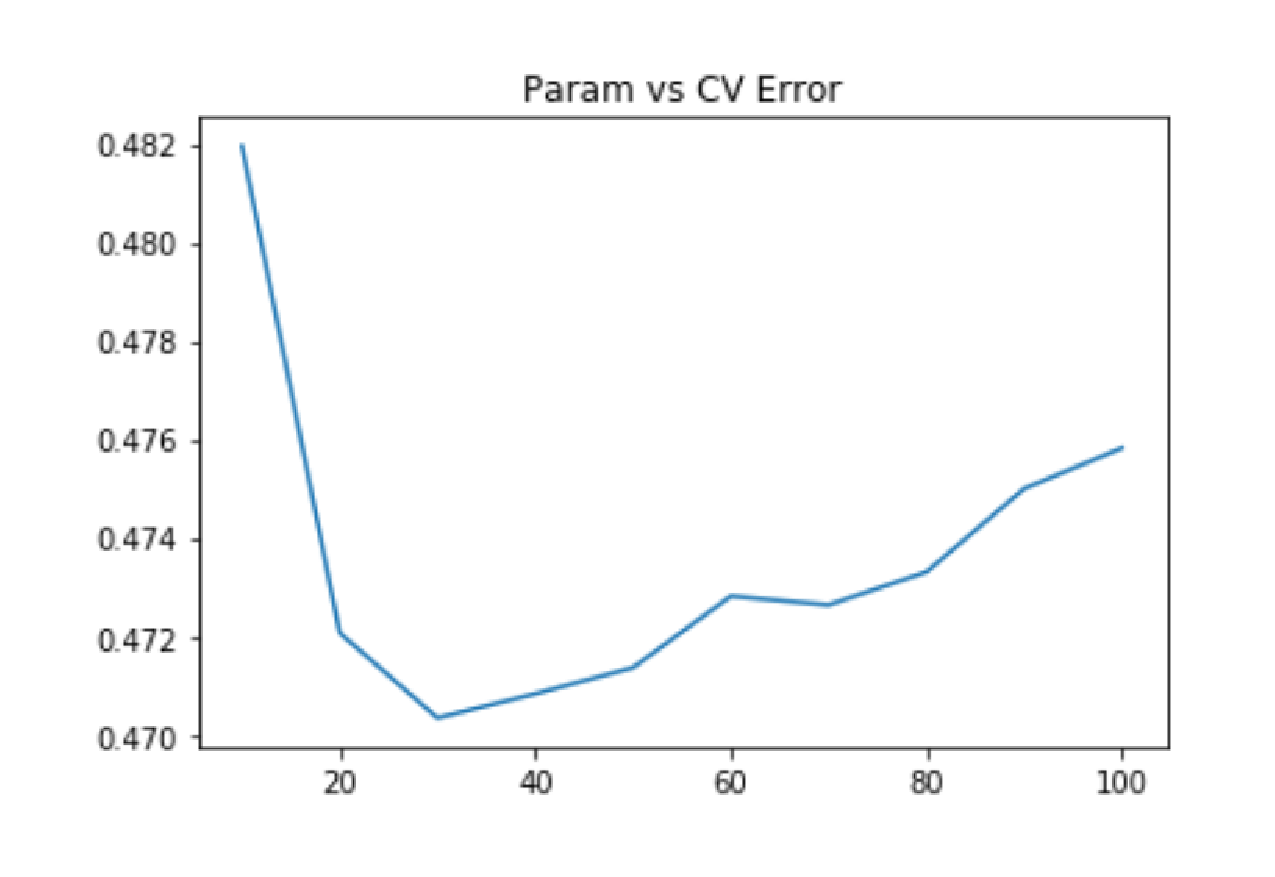
\includegraphics[width=10.5cm, height=5.5cm]{figures/adjust2.eps}
	\caption{Adjusting iterations of Gradient Boosting Regressor
	}\label{straddltimeScale}
\end{figure}
\noindent The result:
	\begin{itemize}
	\item score:0.47101
	\smallskip
	\item rank:347/2123
\end{itemize}

\section{Conclusions} \label{sec-conclusions}
\begin{itemize}
	\item  In this competition, text preprocessing and text feature are important and
	\smallskip 
	\\I know the procedure of dealing NLP problem. Different features that use different method can help the final model predict well. 
	\item  Compare to midterm presentation, MSE decreased from 0.48032 to 0.47101. The reason mainly is more features and different modeling. By adding four features of Word2vec and TFIDF, more information are consideres. Besides, Gradient Boosting Regressor is choosen because of its best performance which means that this model is more suitable for the problem.
	\item  There are some shortcomings. The first team in this competiton is 0.43 and there exists gap. From my point of view, the reason mainly is that some data about product information don't use, and the parameters need to fine-tuned. 
\end{itemize}



% ----------------------------------------------------------------
\newpage
\bibliography{tuliplab,yourbib}
\bibliographystyle{newapa}
%=================================================================

\listoftodos

\end{document}

